\documentclass[main.tex]{subfiles}
\begin{document}

\chapter{Nonparametric Methods}\label{ch:parametrik-olmayan}

For most of the book we have assumed that the data come from a family determined by finitely many parameters. This assumption yields strong results (the Cramér--Rao\index{cramer rao lower bound crlb@Cramér--Rao lower bound (CRLB)} bound, UMP\index{uniformly most powerful ump test@uniformly most powerful (UMP) test} tests, efficiency of the MLE), but if the model is wrong these results may become invalid. \emph{Nonparametric\index{nonparametric methods@nonparametric methods}} methods make only weak assumptions about $F$, such as continuity or symmetry. In this chapter we follow two ideas. First, the distribution of statistics based on the \emph{ranks} of the observations rather than their values does not depend on $F$ under the null hypothesis; this yields tests of exact level (sign, Wilcoxon, Mann--Whitney\index{wilcoxon mann whitney test@Wilcoxon--Mann--Whitney test}, Kolmogorov--Smirnov\index{kolmogorov smirnov test@Kolmogorov--Smirnov test}) and exact confidence intervals for quantiles. Second, $F$ or its density can itself be estimated; the density counterpart of the empirical CDF\index{empirical distribution function@empirical distribution function} of Chapter~\ref{ch:rastgele-degiskenler} is the \emph{kernel density estimate\index{kernel density estimation@kernel density estimation}}. We close the chapter with the question of how much power nonparametric tests lose, i.e.\ with Pitman\index{pitman efficiency@Pitman efficiency} asymptotic relative efficiency\index{asymptotic relative efficiency@asymptotic relative efficiency}. The answer surprises most readers: even for normal data the loss is only about $5\%$.

\section{Definitions}

\begin{definition}[Distribution-Free Statistic]\label{def:dagilimdan-bagimsiz}
For a class $\mathcal F$ of distributions (e.g.\ all continuous distributions), if the distribution of $T(\X)$ when $X_1,\dots,X_n\iid F$ is the same for every $F\in\mathcal F$, then $T$ is called \emph{distribution-free\index{distribution free statistic@distribution-free statistic}} over $\mathcal F$.
\end{definition}

\begin{definition}[Ranks]\label{def:sira}
Let $X_1,\dots,X_n$ be observations without ties. The \emph{rank} of $X_i$ is $R_i=\sum_{j=1}^n\I\{X_j\le X_i\}$; i.e.\ $X_i=X_{(R_i)}$. $\mathbf R=(R_1,\dots,R_n)$ is a permutation of $\{1,\dots,n\}$.
\end{definition}

\begin{definition}[One-Sample Location Tests]\label{def:tek-orneklem-testler}
Let $X_1,\dots,X_n$ be i.i.d.\ from a continuous distribution with median $\theta$; $H_0:\theta=0$.
\begin{itemize}
  \item \emph{Sign statistic:} $S=\sum_i\I\{X_i>0\}$.
  \item \emph{Wilcoxon signed-rank\index{wilcoxon signed rank test@Wilcoxon signed-rank test} statistic:} with $R_i^+$ the rank of $|X_i|$ among $|X_1|,\dots,|X_n|$, $W^+=\sum_iR_i^+\I\{X_i>0\}$.
\end{itemize}
\end{definition}

\begin{definition}[Two Samples: Wilcoxon--Mann--Whitney]\label{def:mann-whitney}\index{wilcoxon mann whitney test@Wilcoxon--Mann--Whitney test|textbf}
Let $X_1,\dots,X_m\iid F$ and $Y_1,\dots,Y_n\iid G$ be independent, $N=m+n$. The sum of the ranks of the $Y_j$ in the combined sample is called the \emph{Wilcoxon rank sum} $W$ \cite{wilcoxon45}, and $U=\sum_{i,j}\I\{X_i<Y_j\}$ the \emph{Mann--Whitney statistic} \cite{mann-whitney47}. $H_0:F=G$ is rejected for large values of $U$ in favour of the alternative that $G$ is shifted to the right.
\end{definition}

\begin{definition}[Kolmogorov--Smirnov Statistics]\label{def:ks}\index{kolmogorov smirnov test@Kolmogorov--Smirnov test|textbf}
One sample: $D_n=\sup_x|\hat F_n(x)-F_0(x)|$, for $H_0:F=F_0$. Two samples: $D_{m,n}=\sup_x|\hat F_m(x)-\hat G_n(x)|$, for $H_0:F=G$.
\end{definition}

% <<fig:ks-mesafe>>
The one-sample statistic is shown in Figure~\ref{fig:ks-mesafe}.

\begin{figure}[ht]
\centering
\begin{tikzpicture}[x=1.7cm,y=4.2cm,font=\small]
\draw[->] (-2.7,0) -- (2.8,0) node[below] {$x$}; \draw[->] (-2.6,0) -- (-2.6,1.12);
\draw (-2.62,1) -- (-2.58,1) node[left] {1}; \draw (-2.62,0.5) -- (-2.58,0.5) node[left] {0.5};
\draw[thick,red!60!black] (-2.600,0.005) -- (-2.542,0.006) -- (-2.483,0.007) -- (-2.425,0.008) -- (-2.366,0.009) -- (-2.308,0.011) -- (-2.249,0.012) -- (-2.191,0.014) -- (-2.133,0.016) -- (-2.074,0.019) -- (-2.016,0.022) -- (-1.957,0.025) -- (-1.899,0.029) -- (-1.840,0.033) -- (-1.782,0.037) -- (-1.724,0.042) -- (-1.665,0.048) -- (-1.607,0.054) -- (-1.548,0.061) -- (-1.490,0.068) -- (-1.431,0.076) -- (-1.373,0.085) -- (-1.315,0.094) -- (-1.256,0.105) -- (-1.198,0.116) -- (-1.139,0.127) -- (-1.081,0.140) -- (-1.022,0.153) -- (-0.964,0.168) -- (-0.906,0.183) -- (-0.847,0.198) -- (-0.789,0.215) -- (-0.730,0.233) -- (-0.672,0.251) -- (-0.613,0.270) -- (-0.555,0.289) -- (-0.497,0.310) -- (-0.438,0.331) -- (-0.380,0.352) -- (-0.321,0.374) -- (-0.263,0.396) -- (-0.204,0.419) -- (-0.146,0.442) -- (-0.088,0.465) -- (-0.029,0.488) -- (0.029,0.512) -- (0.088,0.535) -- (0.146,0.558) -- (0.204,0.581) -- (0.263,0.604) -- (0.321,0.626) -- (0.380,0.648) -- (0.438,0.669) -- (0.497,0.690) -- (0.555,0.711) -- (0.613,0.730) -- (0.672,0.749) -- (0.730,0.767) -- (0.789,0.785) -- (0.847,0.802) -- (0.906,0.817) -- (0.964,0.832) -- (1.022,0.847) -- (1.081,0.860) -- (1.139,0.873) -- (1.198,0.884) -- (1.256,0.895) -- (1.315,0.906) -- (1.373,0.915) -- (1.431,0.924) -- (1.490,0.932) -- (1.548,0.939) -- (1.607,0.946) -- (1.665,0.952) -- (1.724,0.958) -- (1.782,0.963) -- (1.840,0.967) -- (1.899,0.971) -- (1.957,0.975) -- (2.016,0.978) -- (2.074,0.981) -- (2.133,0.984) -- (2.191,0.986) -- (2.249,0.988) -- (2.308,0.989) -- (2.366,0.991) -- (2.425,0.992) -- (2.483,0.993) -- (2.542,0.994) -- (2.600,0.995) node[above left] {$F_0=\Phi$};
\draw[very thick,blue!60!black] (-2.600,0.0000) -- (-1.786,0.0000);
\fill[blue!60!black] (-1.786,0.0833) circle (1.3pt);
\draw[very thick,blue!60!black] (-1.786,0.0833) -- (-1.083,0.0833);
\fill[blue!60!black] (-1.083,0.1667) circle (1.3pt);
\draw[very thick,blue!60!black] (-1.083,0.1667) -- (-0.803,0.1667);
\fill[blue!60!black] (-0.803,0.2500) circle (1.3pt);
\draw[very thick,blue!60!black] (-0.803,0.2500) -- (-0.800,0.2500);
\fill[blue!60!black] (-0.800,0.3333) circle (1.3pt);
\draw[very thick,blue!60!black] (-0.800,0.3333) -- (-0.224,0.3333);
\fill[blue!60!black] (-0.224,0.4167) circle (1.3pt);
\draw[very thick,blue!60!black] (-0.224,0.4167) -- (-0.047,0.4167);
\fill[blue!60!black] (-0.047,0.5000) circle (1.3pt);
\draw[very thick,blue!60!black] (-0.047,0.5000) -- (0.359,0.5000);
\fill[blue!60!black] (0.359,0.5833) circle (1.3pt);
\draw[very thick,blue!60!black] (0.359,0.5833) -- (0.584,0.5833);
\fill[blue!60!black] (0.584,0.6667) circle (1.3pt);
\draw[very thick,blue!60!black] (0.584,0.6667) -- (0.638,0.6667);
\fill[blue!60!black] (0.638,0.7500) circle (1.3pt);
\draw[very thick,blue!60!black] (0.638,0.7500) -- (0.834,0.7500);
\fill[blue!60!black] (0.834,0.8333) circle (1.3pt);
\draw[very thick,blue!60!black] (0.834,0.8333) -- (1.511,0.8333);
\fill[blue!60!black] (1.511,0.9167) circle (1.3pt);
\draw[very thick,blue!60!black] (1.511,0.9167) -- (1.687,0.9167);
\fill[blue!60!black] (1.687,1.0000) circle (1.3pt);
\draw[very thick,blue!60!black] (1.687,1) -- (2.6,1);
\draw[{Latex}-{Latex},orange!80!black,thick] (0.359,0.5000) -- (0.359,0.6401) node[midway,left,font=\footnotesize,fill=white,inner sep=1pt,xshift=-3pt] {$D_n$};
\node[blue!60!black,anchor=west] at (0.9,0.62) {$\hat F_n$};
\end{tikzpicture}
\caption{The Kolmogorov--Smirnov statistic. The empirical CDF $\hat F_n$ (step function) of $n=12$ observations from $\Normal(0,1)$ and the null CDF $F_0=\Phi$. $D_n$ is the largest vertical distance between the two curves; the largest distance always occurs just before or just after a step.}\label{fig:ks-mesafe}
\end{figure}
% <</fig:ks-mesafe>>

\begin{definition}[Kernel Density Estimator]\label{def:kde}
Let $K\ge0$ be a symmetric \emph{kernel} with $\int K=1$, $\int uK(u)du=0$, $\mu_2(K)=\int u^2K(u)du<\infty$ and $R(K)=\int K^2<\infty$, and let $h>0$ be the \emph{bandwidth\index{bandwidth@bandwidth}}. The kernel density estimator\index{kernel density estimation@kernel density estimation} \cite{rosenblatt56,parzen62} is defined as
\[
\hat f_h(x)=\frac1{nh}\sum_{i=1}^nK\Big(\frac{x-X_i}{h}\Big) .
\]
Each observation is replaced by a small ``bump'' of width $h$ centred at it. As the error criterion the \emph{mean integrated squared error} is used: $\mathrm{MISE}(h)=\E\int(\hat f_h-f)^2$.
\end{definition}

\begin{definition}[Pitman Asymptotic Relative Efficiency]\label{def:pitman}\index{pitman efficiency@Pitman efficiency|textbf}
Suppose two sequences of level-$\alpha$ tests require $n_1$ and $n_2$ observations, respectively, to achieve the same limiting power against alternatives approaching $\theta_0$ at the rate $\theta_n=\theta_0+h/\sqrt n$. The limit of the ratio $n_2/n_1$ is called the \emph{Pitman ARE} of the first test relative to the second. It is the testing counterpart of the estimator ARE of Chapter~\ref{ch:mle-asimptotik}.
\end{definition}

\section{Main Theorems and Proofs}

\begin{theorem}[Distribution-Free Confidence Interval for Quantiles]\label{thm:kantil-ga}
Let $X_1,\dots,X_n\iid F$ with $F$ continuous, and let $\xi_p$ be a quantile with $F(\xi_p)=p$. For $r<s$,
\[
\P\big(X_{(r)}\le\xi_p<X_{(s)}\big)=\sum_{j=r}^{s-1}\binom nj p^j(1-p)^{n-j}.
\]
This probability does not depend on $F$; hence $[X_{(r)},X_{(s)}]$ is a confidence interval for $\xi_p$ with known exact coverage probability.
\end{theorem}
\begin{proof}
$B=\#\{i:X_i\le\xi_p\}\sim\text{Bin}(n,p)$, because $\P(X_i\le\xi_p)=F(\xi_p)=p$. The event $X_{(r)}\le\xi_p$ is ``at least $r$ observations are less than or equal to $\xi_p$'', i.e.\ the event $\{B\ge r\}$. Similarly $\{X_{(s)}\le\xi_p\}=\{B\ge s\}$. Hence $\{X_{(r)}\le\xi_p<X_{(s)}\}=\{r\le B\le s-1\}$. Since by continuity $\P(X_{(s)}=\xi_p)=0$, whether the interval is taken closed or open does not change the probability.
\end{proof}

\begin{theorem}[Distribution of the Rank Vector]\label{thm:sira-dagilim}
If $X_1,\dots,X_n\iid F$ with $F$ continuous, then
\begin{enumerate}
  \item there are a.s.\ no ties, and $\mathbf R$ is uniformly distributed over the $n!$ permutations of $\{1,\dots,n\}$;
  \item $\mathbf R$ is independent of the vector of order statistics\index{order statistics@order statistics} $(X_{(1)},\dots,X_{(n)})$.
\end{enumerate}
Consequently, every function of the ranks is distribution-free\index{distribution free statistic@distribution-free statistic} over all continuous distributions.
\end{theorem}
\begin{proof}
(1) For $i\ne j$, $\P(X_i=X_j)=\int\P(X_i=x)\,dF(x)=0$, because a continuous distribution has no atoms; a finite union also has probability zero. (2) For a permutation $\sigma$, $(X_{\sigma(1)},\dots,X_{\sigma(n)})$ has the same distribution as $(X_1,\dots,X_n)$ by the i.i.d.\ structure (exchangeability\index{exchangeability@exchangeability}). The event $\mathbf R=\mathbf r$ is the event ``the position of $X_i$ in the ordered vector is $r_i$''. A permutation leaves the ordered vector unchanged but carries the rank vector to another permutation. Hence for every measurable $B$ and any two permutations $\mathbf r,\mathbf r'$,
\[
\P\big(\mathbf R=\mathbf r,\ (X_{(1)},\dots,X_{(n)})\in B\big)=\P\big(\mathbf R=\mathbf r',\ (X_{(1)},\dots,X_{(n)})\in B\big).
\]
Summing over the $n!$ permutations, each term equals $\P\big((X_{(\cdot)})\in B\big)/n!$. Taking $B$ to be the whole space gives the uniformity in (1), and for general $B$ the product form, i.e.\ independence.
\end{proof}

\begin{theorem}[Null Distribution of the Wilcoxon Signed-Rank Statistic]\label{thm:wilcoxon-isaretli}
If $X_1,\dots,X_n$ are i.i.d.\ from a continuous distribution symmetric about $0$, then
\[
W^+\overset{d}{=}\sum_{j=1}^n j\,B_j,\qquad B_1,\dots,B_n\iid\text{Bernoulli}(1/2),
\]
and $\E W^+=\frac{n(n+1)}4$, $\Var W^+=\frac{n(n+1)(2n+1)}{24}$. Moreover $S\sim\text{Bin}(n,1/2)$.
\end{theorem}
\begin{proof}
Under symmetry and continuity, $\I\{X_i>0\}$ and $|X_i|$ are independent: for every $t\ge0$, $\P(X_i>0,|X_i|\le t)=\P(0<X_i\le t)=\frac12\P(|X_i|\le t)$, and $\P(X_i>0)=\frac12$. Hence the signs $\epsilon_i=\I\{X_i>0\}$ are $\text{Bernoulli}(1/2)$ variables independent of the vector $(|X_1|,\dots,|X_n|)$ and of each other. If $B_j$ denotes the sign of the observation in position $j$ of the ordered $|X|$'s, the $B_j$ are also i.i.d.\ $\text{Bernoulli}(1/2)$, independent of the ordering of the $(|X_i|)$, and $W^+=\sum_jjB_j$. Moments: $\E W^+=\frac12\sum_jj=\frac{n(n+1)}4$, $\Var W^+=\frac14\sum_jj^2=\frac{n(n+1)(2n+1)}{24}$. Since $S=\sum_iB_i$, the last claim is clear.
\end{proof}

\begin{theorem}[Null Moments of the Wilcoxon--Mann--Whitney Statistic]\label{thm:mann-whitney}\index{wilcoxon mann whitney test@Wilcoxon--Mann--Whitney test}
Under $H_0:F=G$ ($F$ continuous),
\[
U=W-\frac{n(n+1)}2,\qquad\E W=\frac{n(N+1)}2,\qquad\Var W=\Var U=\frac{mn(N+1)}{12}.
\]
\end{theorem}
\begin{proof}
\emph{Identity.} Let $Y_{(j)}$ be the $j$-th smallest of the $Y$'s. Its rank in the combined sample is the number of $Y$'s smaller than it ($j-1$), plus the number of $X$'s smaller than it, plus itself ($1$): $j+\#\{i:X_i<Y_{(j)}\}$. Summing over $j$ gives $W=\frac{n(n+1)}2+U$.

\emph{Moments.} Under $H_0$ the $N$ observations are i.i.d., so by Theorem~\ref{thm:sira-dagilim} the ranks of the $Y$'s form a random subset of size $n$ drawn without replacement from $\{1,\dots,N\}$. For sampling without replacement from a finite population, the expected value of the sum is $n\bar r$ and its variance $n\sigma_r^2\frac{N-n}{N-1}$, where the population mean is $\bar r=\frac{N+1}2$ and the population variance $\sigma_r^2=\frac{N^2-1}{12}$. Hence $\E W=\frac{n(N+1)}2$ and $\Var W=n\frac{(N-1)(N+1)}{12}\cdot\frac{m}{N-1}=\frac{mn(N+1)}{12}$.
\end{proof}

\begin{remark}
$U/(mn)$ is an unbiased estimator\index{unbiased estimator@unbiased estimator} of $\P(X<Y)$; the area under the ROC curve (AUC) is exactly this quantity. Under $H_0$, $\P(X<Y)=\frac12$. The alternatives against which the test is consistent are those with $\P(X<Y)\ne\frac12$; that is, the Mann--Whitney test does not answer the question ``are the means equal?'' but the question ``is an observation chosen at random from one group more likely to be larger than one from the other?''.
\end{remark}

\begin{theorem}[The KS Statistic Is Distribution-Free]\label{thm:ks}\index{kolmogorov smirnov test@Kolmogorov--Smirnov test}
If $F_0$ is continuous and $H_0:F=F_0$ is true, the distribution of $D_n$ equals that of $\sup_{u\in[0,1]}|\hat G_n(u)-u|$ built from $U_i\iid\text{Uniform}(0,1)$; i.e.\ it does not depend on $F_0$. Moreover \cite{kolmogorov33b}
\[
\lim_{n\to\infty}\P\big(\sqrt nD_n\le t\big)=1-2\sum_{k=1}^\infty(-1)^{k-1}e^{-2k^2t^2},\qquad t>0 .
\]
\end{theorem}
\begin{proof}[Proof (first part)]
Let $U_i=F_0(X_i)\iid\text{Uniform}(0,1)$ (Theorem~\ref{thm:pit}) and let $\hat G_n$ be their empirical CDF\index{empirical distribution function@empirical distribution function}. Since $F_0$ is non-decreasing, $X_i\le x\Rightarrow U_i\le F_0(x)$; conversely, $X_i>x$ while $U_i\le F_0(x)$ requires $F_0$ to be constant on $[x,X_i]$, an event of probability zero. Hence a.s., for every $x$, $\hat F_n(x)=\hat G_n(F_0(x))$ and
\[
D_n=\sup_x\big|\hat G_n(F_0(x))-F_0(x)\big|=\sup_{u\in(0,1)}\big|\hat G_n(u)-u\big|,
\]
because the range of a continuous $F_0$ contains $(0,1)$; at the endpoints the difference is zero. The limit distribution comes from the convergence of the process $\sqrt n(\hat G_n-u)$ to a Brownian bridge and from the distribution of the supremum of a Brownian bridge; see \cite[Chapter~19]{vdv}.
\end{proof}

\begin{theorem}[Bias, Variance and Optimal Bandwidth of the Kernel Estimator]\label{thm:kde}\index{bandwidth@bandwidth}
Let $f$ be twice continuously differentiable with $f''$ bounded. As $h\to0$ and $nh\to\infty$, for every $x$,
\[
\E\hat f_h(x)-f(x)=\frac{h^2}2\mu_2(K)f''(x)+o(h^2),\qquad\Var\hat f_h(x)=\frac{f(x)R(K)}{nh}+o\Big(\frac1{nh}\Big).
\]
Under suitable integrability conditions the leading terms of the integrated squared error are
\[
\mathrm{AMISE}(h)=\frac{h^4}4\mu_2(K)^2R(f'')+\frac{R(K)}{nh} ;
\]
the bandwidth minimising this and the resulting error are
\[
h^*=\Big[\frac{R(K)}{\mu_2(K)^2R(f'')\,n}\Big]^{1/5},\qquad\mathrm{AMISE}(h^*)=\frac54\big(\mu_2(K)^2R(f'')\big)^{1/5}R(K)^{4/5}\,n^{-4/5}.
\]
\end{theorem}
\begin{proof}
\emph{Bias.} With the variable $u=(x-y)/h$, $\E\hat f_h(x)=\int\frac1hK\big(\frac{x-y}h\big)f(y)\,dy=\int K(u)f(x-hu)\,du$. By Taylor expansion, for some $\xi$ between $x$ and $x-hu$, $f(x-hu)=f(x)-huf'(x)+\frac{h^2u^2}2f''(\xi)$. Since $\int K=1$ and $\int uK=0$,
\[
\E\hat f_h(x)-f(x)=\frac{h^2}2\int u^2K(u)f''(\xi_{u,h})\,du .
\]
Since $f''$ is continuous and bounded and $u^2K(u)$ is integrable, by dominated convergence the integral tends to $\mu_2(K)f''(x)$.

\emph{Variance.} $\hat f_h(x)$ is the mean of the i.i.d.\ variables $Z_i=\frac1hK(\frac{x-X_i}h)$: $\Var\hat f_h(x)=\frac1n\big(\E Z_1^2-(\E Z_1)^2\big)$. With the same change of variables $\E Z_1^2=\frac1h\int K(u)^2f(x-hu)\,du=\frac1h\big(f(x)R(K)+o(1)\big)$ and $(\E Z_1)^2=O(1)$; hence $\Var\hat f_h(x)=\frac{f(x)R(K)}{nh}+O(\frac1n)$, and as $h\to0$, $O(1/n)=o(1/(nh))$.

\emph{AMISE\index{mise@MISE}.} $\mathrm{MSE}=\text{bias}^2+\text{variance}$; integrate over $x$ and use $\int f=1$. With $A=\mu_2^2R(f'')/4$ and $B=R(K)/n$, the derivative of $Ah^4+B/h$ is $4Ah^3-B/h^2$, which vanishes at $h^5=B/(4A)$; this is $h^*$. At this point $B/h=4Ah^4$, so the value is $5Ah^{*4}=\frac54(4A)^{1/5}B^{4/5}$.
\end{proof}

\begin{theorem}[Pitman Efficiencies]\label{thm:pitman-are}\index{pitman efficiency@Pitman efficiency}
Let $X_i=\theta+\varepsilon_i$, with the $\varepsilon_i$ i.i.d., symmetric about $0$, with density $f$ and variance $\sigma^2$; $H_0:\theta=0$. Under sufficient regularity conditions\index{regularity conditions@regularity conditions},
\[
\mathrm{ARE}(S,t)=4\sigma^2f(0)^2,\qquad\mathrm{ARE}(W^+,t)=12\sigma^2\Big(\int f^2\Big)^2 .
\]
\end{theorem}
\begin{proof}[Main idea of the proof]
By Noether's theorem \cite[Chapter~14]{vdv}, if $\sqrt n\big(T_n-\mu(\theta)\big)/\tau(\theta)\dto\Normal(0,1)$ holds uniformly along local alternatives, the local power of a test is determined only by its \emph{efficacy} $e=\mu'(0)^2/\tau(0)^2$, and the ARE is the ratio of efficacies. For the three tests:
\begin{itemize}
  \item $t$: $T=\bar X$, $\mu(\theta)=\theta$, $\tau^2=\sigma^2$; $e_t=1/\sigma^2$.
  \item Sign: $T=S/n$, $\mu(\theta)=\P(\varepsilon>-\theta)=F(\theta)$, $\mu'(0)=f(0)$, $\tau^2(0)=\frac14$; $e_S=4f(0)^2$.
  \item Wilcoxon: $W^+/\binom n2$ is asymptotically equivalent to the average of $\I\{X_i+X_j>0\}$ over pairs $i<j$ (a $U$-statistic). $\mu(\theta)=\P(\varepsilon_1+\varepsilon_2>-2\theta)$; since the density of $\varepsilon_1+\varepsilon_2$ at $0$ is $\int f(x)f(-x)dx=\int f^2$, $\mu'(0)=2\int f^2$. The asymptotic variance of the $U$-statistic is $4\Var\big(F(\varepsilon_1)\big)=\frac4{12}=\frac13$. Hence $e_W=12(\int f^2)^2$.
\end{itemize}
Taking the ratios gives the result.
\end{proof}

\section{Worked Examples}

\begin{example}[Exact Confidence Interval for the Median]\label{ex:medyan-ga}
$n=20$, $p=\frac12$. By Theorem~\ref{thm:kantil-ga}, the coverage probability of $[X_{(6)},X_{(15)}]$ is $\P(6\le B\le14)=0.9586$, and that of $[X_{(7)},X_{(14)}]$ is $0.8847$. Because of the discrete binomial structure, exactly $95\%$ cannot be attained; the narrowest symmetric interval not falling below $95\%$ is $[X_{(6)},X_{(15)}]$. This interval requires no assumption about $F$ other than continuity; it is valid for Cauchy data too.
\end{example}

\begin{example}[Pitman ARE Values]\label{ex:are-degerleri}
The formulas of Theorem~\ref{thm:pitman-are} give:
\begin{center}
\begin{tabular}{lccc}
\toprule
Distribution & $\int f^2$ & $\mathrm{ARE}(W^+,t)$ & $\mathrm{ARE}(S,t)$\\
\midrule
Normal $\Normal(0,\sigma^2)$ & $\frac1{2\sigma\sqrt\pi}$ & $3/\pi\approx0.955$ & $2/\pi\approx0.637$\\
Logistic & $\frac1{6s}$ & $\pi^2/9\approx1.097$ & $\pi^2/12\approx0.822$\\
Laplace (scale $b$) & $\frac1{4b}$ & $1.5$ & $2$\\
Uniform $(-1,1)$ & $\frac12$ & $1$ & $1/3$\\
\bottomrule
\end{tabular}
\end{center}
(For the logistic, $s$ is the scale parameter, $\sigma^2=\pi^2s^2/3$ and $f(0)=\frac1{4s}$.) Hodges and Lehmann \cite{hodges-lehmann56} showed that over the class of symmetric continuous densities $\mathrm{ARE}(W^+,t)\ge\frac{108}{125}=0.864$, and that there is no upper bound. That is, relative to the $t$-test the Wilcoxon test loses at most $14\%$ efficiency in the worst case, but can gain without limit. The sign test\index{sign test@sign test}, on the other hand, wastes a third of the observations for normal data.
\end{example}

\begin{example}[Mann--Whitney: Exact Small-Sample Distribution]\label{ex:mw-kesin}
$m=n=3$, $N=6$. Under $H_0$ the ranks of the $Y$'s are each of the $\binom63=20$ subsets with probability $\frac1{20}$. $W$ takes values from $6$ to $15$; $\P(W=15)=\P(W=6)=\frac1{20}$. Hence the one-sided test with $\alpha=0.05$ rejects only if all the $Y$'s are larger than all the $X$'s. In very small samples, the attainable levels of nonparametric\index{nonparametric methods@nonparametric methods} tests form a coarse grid.
\end{example}

\section{Computational Applications}

\subsection{Level and Power of Three Tests}
With $n=30$ observations from four distributions scaled to variance $1$, we compute the rejection rates of the $t$, Wilcoxon signed-rank\index{wilcoxon signed rank test@Wilcoxon signed-rank test} and sign tests\index{sign test@sign test} under $\theta=0$ (level) and $\theta=0.5$ (power) with $M=4000$ replications.

\pycode{code/ch21/c21_1_t_wilcoxon_sign_power.py}
\begin{lstlisting}[style=output]
Distrib.| theta | t-test  | Wilcoxon | sign
Normal  |  0.0  |  0.057  |  0.057   | 0.044
Normal  |  0.5  |  0.764  |  0.745   | 0.561
Laplace |  0.0  |  0.050  |  0.057   | 0.049
Laplace |  0.5  |  0.753  |  0.837   | 0.818
t_3     |  0.0  |  0.043  |  0.053   | 0.041
t_3     |  0.5  |  0.825  |  0.935   | 0.898
Uniform |  0.0  |  0.050  |  0.046   | 0.039
Uniform |  0.5  |  0.761  |  0.689   | 0.342
Theoretical Pitman ARE (Wilcoxon/t, sign/t): {'Normal': (0.955, 0.637), 'Laplace': (1.5, 2.0), 'Uniform': (1.0, 0.333)}
\end{lstlisting}

The power ranking follows the Pitman\index{pitman efficiency@Pitman efficiency} ARE table. For normal data $t$ is most powerful, but the loss of Wilcoxon is small; the sign test lags clearly behind. For heavy-tailed distributions such as the Laplace and $t_3$, both nonparametric\index{nonparametric methods@nonparametric methods} tests beat $t$. For the uniform distribution the power of the sign test collapses ($\mathrm{ARE}=1/3$). Under the null hypothesis all three tests approximately keep the level. The sign test is slightly conservative, because the binomial distribution is discrete and the exact $5\%$ level is not attainable.

\subsection{Kolmogorov--Smirnov and the Lilliefors Problem}

\pycode{code/ch21/c21_2_kolmogorov_smirnov.py}
\begin{lstlisting}[style=output]
Quantiles        : [0.5, 0.9, 0.95, 0.99]
D_n, normal data : [0.1773 0.2633 0.2924 0.3512]
D_n, expon. data : [0.1775 0.264  0.2942 0.3498]
Exact (kstwo)    : [0.1773 0.2647 0.2941 0.3524]
Asymptotic K/sqrt(n): [0.1851 0.2737 0.3037 0.3639]
H0 true, parameters estimated: rejection rate (target 0.05) = 0.0000
0.95 quantile of the estimated statistic = 0.1909 (KS critical value 0.2941)
\end{lstlisting}

The quantiles of $D_n$ computed from normal and exponential data agree within Monte Carlo error and match the exact distribution (\texttt{kstwo}): the distribution-freeness\index{distribution free statistic@distribution-free statistic} claim of Theorem~\ref{thm:ks}. At $n=20$ the asymptotic Kolmogorov distribution slightly overstates the quantiles. The last two lines show a common mistake. If, when testing normality, $\mu$ and $\sigma$ are estimated from the data and the standard KS\index{kolmogorov smirnov test@Kolmogorov--Smirnov test} critical values are used, the test almost never rejects. Since the estimated distribution is ``too close'' to the data, $D_n$ is systematically smaller. The correct critical values (Lilliefors\index{lilliefors problem@Lilliefors problem} \cite{lilliefors67}) must be obtained by simulation or by the parametric bootstrap\index{bootstrap@bootstrap!parametric@parametric} (Chapter~\ref{ch:bootstrap}).

\subsection{Kernel Density Estimation: Bandwidth and Rate of Convergence}
For a bimodal mixture density we plot the Gaussian-kernel estimator\index{kernel density estimation@kernel density estimation} with different values of $h$, and measure by Monte Carlo the AMISE\index{mise@MISE}-optimal $h^*$ of Theorem~\ref{thm:kde} and the rate at which the MISE decreases with $n$.

\pycode{code/ch21/c21_3_kernel_density.py}
\begin{lstlisting}[style=output]
R(f'') = 1.6075
    n | h_opt  | MISE (MC) | AMISE theory
  100 | 0.2811 | 0.009296  | 0.012545
  400 | 0.2130 | 0.003604  | 0.004138
 1600 | 0.1614 | 0.001121  | 0.001365
 6400 | 0.1224 | 0.000412  | 0.000450
slope of log MISE ~ log n = -0.759 (theory: -0.8; parametric rate: -1)
n=200: Silverman h = 0.592 | AMISE-optimal h = 0.245
\end{lstlisting}

\begin{figure}[h]
\centering
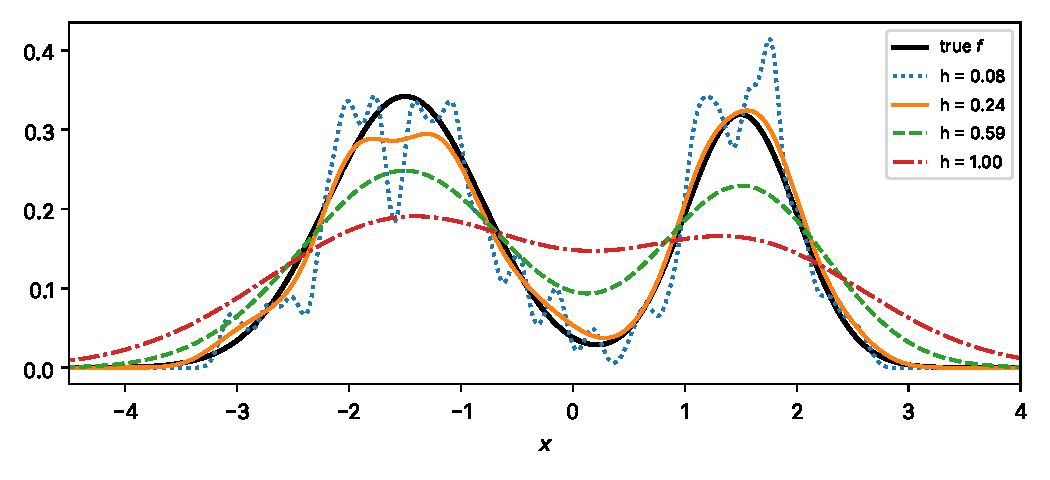
\includegraphics[width=0.85\textwidth]{figures/cekirdek_bant.pdf}
\caption{Kernel density estimates with $n=200$ observations. Small $h$ (dotted) is noisy; large $h$ (dash-dotted) is biased enough to merge the two modes. Silverman's rule (dashed), derived for the normal distribution, oversmooths the bimodal density.}
\end{figure}

The log--log slope of the MISE is about $-0.76$, close to the theoretical $-4/5$. For small $n$ the slope is somewhat flatter because of the terms neglected by AMISE. This rate is slower than the $1/n$ of parametric models: estimating a density locally at every point is harder than estimating finitely many parameters. The rate $n^{-4/5}$ is the minimax\index{minimax rule@minimax rule} rate over the class of twice-differentiable densities (Chapter~\ref{ch:karar}). That Silverman\index{silverman s rule@Silverman's rule}'s rule gives $0.59$, far from the optimal $0.25$, is a reminder that the ``rule'' rests on a normality assumption.

\subsection{Real Data: Student's Sleep Data}\label{sec:uyku}
The data in which Cushny and Peebles measured the effect of two sleeping drugs on 10 patients \cite{cushny-peebles05} are the example Student\index{t distribution student@$t$ distribution (Student)} used in the paper that introduced the $t$ distribution \cite{student08}. Every patient took both drugs; the measurement is the extra sleep produced by the drug (hours). Since patients differ a lot, the analysis must use the differences $d_i=\text{drug}_2-\text{drug}_1$. The data have two small features: one difference is zero and two differences are equal. So in the sign and Wilcoxon tests the zero difference is dropped, the equal differences get midranks, and the null distribution is computed exactly (conditionally) by enumerating the $2^9$ sign assignments. The code compares the paired $t$ test (Chapter~\ref{ch:guven}), the sign test, the Wilcoxon signed-rank test and the sign-flip permutation test\index{permutation test@permutation test}; it then shows the wrong analysis that ignores the pairing.

\pycode{code/ch21/c21_4_sleep_data_real_data.py}
\begin{lstlisting}[style=output]
differences d = [1.2 2.4 1.3 1.3 0.  1.  1.8 0.8 4.6 1.4] | mean = 1.58, s = 1.230, median = 1.30
paired t: t = 4.062, p = 0.0028, 95% CI = [0.70, 2.46]
sign test: 9/9 positive, p = 0.0039
Wilcoxon: W+ = 45.0 (largest possible value 45), exact p = 0.0039
permutation: 2^10 = 1024 sign assignments, p = 0.0039
two-sample t (wrong): t = 1.861, p = 0.0792 | Corr(drug1, drug2) = 0.795
\end{lstlisting}

The four valid analyses reach the same conclusion: the second drug increases extra sleep by $1.58$ hours on average ($95\%$ CI $[0.70,\,2.46]$). All nine nonzero differences are positive. So the three distribution-free tests give the smallest $p$-value attainable at this sample size: $2/2^9\approx0.0039$. Distribution-free tests have a floor for the $p$-value at small $n$; a smaller value can only be obtained with an extra assumption such as normality ($0.0028$ for the $t$ test). The two-sample $t$ test that ignores the pairing misses the effect ($p=0.079$). The reason is that the two measurements on the same patient are strongly correlated ($r=0.80$): some patients sleep a lot with both drugs, others little. Since the variance of the differences is $s_1^2+s_2^2-2rs_1s_2$, pairing removes this between-patient variability (Exercise~\ref{exr:21-5}). This is the value of pairing in experimental design.

\section{Comments and Notes}

\begin{remark}[Ties]
In real data, ties arise from rounding of measurements. In that case tied observations receive their average rank, and the null distribution is computed conditionally (given the tie structure) by permutation. A tie correction is added to the variance formulas. In one-sample tests, observations with $X_i=0$ are usually discarded.
\end{remark}

\begin{remark}[The Hodges--Lehmann Estimator and Confidence Intervals]
By the duality\index{test interval duality@test--interval duality} of Chapter~\ref{ch:guven}, every test produces a confidence interval and a point estimate. Inverting the Wilcoxon signed-rank\index{wilcoxon signed rank test@Wilcoxon signed-rank test} test gives the confidence interval built from the \emph{Walsh averages} $(X_i+X_j)/2$, $i\le j$. The median of these averages is the \emph{Hodges--Lehmann\index{hodges lehmann estimator@Hodges--Lehmann estimator} estimator}. Its ARE is the same as that of the Wilcoxon test: $0.955$ for normal data, and much better than the mean for heavy tails.
\end{remark}

\begin{remark}[The Price of Nonparametric Inference]
Rank tests lose almost no power against shift alternatives. In estimating densities and regression functions, by contrast, the price is paid in the rate of convergence: $n^{-4/5}$ becomes $n^{-4/(4+d)}$ in $d$ dimensions. This \emph{curse of dimensionality} explains why high-dimensional nonparametric\index{nonparametric methods@nonparametric methods} estimation requires structural assumptions (additivity, sparsity).
\end{remark}

% --- CHAPTER SUMMARY ---
\section{Chapter Summary}
\begin{summary}
\begin{itemize}
  \item Under a continuous $F$ the rank vector is uniformly distributed over all permutations (Theorem~\ref{thm:sira-dagilim}). Statistics based on ranks are therefore distribution-free.
  \item Confidence intervals for quantiles are built from order statistics and binomial probabilities without any distributional assumption (Theorem~\ref{thm:kantil-ga}).
  \item Location tests: the sign test, the Wilcoxon signed-rank test (Theorem~\ref{thm:wilcoxon-isaretli}) and, for two samples, the Wilcoxon--Mann--Whitney test (Theorem~\ref{thm:mann-whitney}).
  \item Pitman efficiency (Theorem~\ref{thm:pitman-are}): the Wilcoxon test has $95.5\%$ of the efficiency of the $t$-test for normal data and never falls below $0.864$ for any symmetric continuous distribution. For heavy tails it beats $t$.
  \item The Kolmogorov--Smirnov statistic is distribution-free (Theorem~\ref{thm:ks}). If parameters are estimated from the data this property is lost (the Lilliefors problem).
  \item In kernel density estimation the bias is of order $O(h^2)$ and the variance of order $O(1/(nh))$. The optimal bandwidth is $h^*\propto n^{-1/5}$, and the MISE decreases at the rate $n^{-4/5}$ (Theorem~\ref{thm:kde}).
\end{itemize}
\end{summary}
% --- END OF CHAPTER SUMMARY ---

\paragraph{Further reading.} \cite{lehmann75}, \cite{wasserman06}; for kernel methods, \cite{silverman86}; for asymptotic theory, \cite[Chapters~13--14 and 19]{vdv}.

\section{Exercises}

\begin{exercise}\label{exr:21-1}
Let $X_1,\dots,X_n\iid F$ with $F$ continuous, $p\in(0,1)$ fixed and $k=\lceil np\rceil$. Using $F(X_{(k)})\sim\text{Beta}(k,n-k+1)$ (Example~\ref{ex:uniform-sira}), show that $F(X_{(k)})\pto p$. Deduce that $X_{(k)}\pto\xi_p$ if $f(\xi_p)>0$.
\hfill\hyperref[coz:21-1]{\footnotesize$\rightarrow$\,Solution}
\end{exercise}

\begin{exercise}\label{exr:21-2}
With $n=25$ observations, find the narrowest symmetric interval $[X_{(r)},X_{(n+1-r)}]$ for the median whose coverage does not fall below $95\%$, and compute its exact coverage probability. Derive the rule $r\approx\frac n2-z_{\alpha/2}\frac{\sqrt n}2$ from the normal approximation.
\hfill\hyperref[coz:21-2]{\footnotesize$\rightarrow$\,Solution}
\end{exercise}

\begin{exercise}\label{exr:21-3}
For $m=n=3$, derive the exact null distribution of $W$, compute $\E W$ and $\Var W$ from this distribution, and compare with Theorem~\ref{thm:mann-whitney}. Show that $U/(mn)$ is unbiased for $\P(X<Y)$.
\hfill\hyperref[coz:21-3]{\footnotesize$\rightarrow$\,Solution}
\end{exercise}

\begin{exercise}\label{exr:21-4}
For the Gaussian kernel and the true density $\Normal(\mu,\sigma^2)$, compute the $h^*$ of Theorem~\ref{thm:kde} and show that $h^*=(4/3)^{1/5}\sigma n^{-1/5}\approx1.06\,\sigma n^{-1/5}$ (Silverman's rule). ($R(K)=\frac1{2\sqrt\pi}$, $\mu_2=1$ and $\int(\phi_\sigma'')^2=\frac{3}{8\sqrt\pi\sigma^5}$.)
\hfill\hyperref[coz:21-4]{\footnotesize$\rightarrow$\,Solution}
\end{exercise}

\begin{exercise}\label{exr:21-5}
In the sleep data the sample standard deviations of the two drugs are $s_1=1.789$ and $s_2=2.002$, and their correlation is $r=0.795$. Show that the standard deviation of the differences is $s_d=\sqrt{s_1^2+s_2^2-2rs_1s_2}$ and compute it. Compare the standard error of $\bar d$ in the paired analysis with $\sqrt{(s_1^2+s_2^2)/n}$ used in the two-sample analysis. When does pairing bring no gain?
\hfill\hyperref[coz:21-5]{\footnotesize$\rightarrow$\,Solution}
\end{exercise}

\chapterlinks{21}

\end{document}
